\chapter{Khảo sát dữ liệu và tiền xử lý dữ liệu}
\section{Các tập dữ liệu sử dụng}
Để mô hình xây dựng đủ độ chính xác và có tính ứng dụng thực tế cũng như có thể được đánh giá khách quan, chúng tôi sử dụng các tập dữ liệu bệnh nhân thật đã được các y bác sĩ có chuyên môn tiến hành phân đoạn và công bố rộng rãi tại nhiều cuộc thi, hội nghị trên toàn thế giới. Cụ thể chúng tôi sử dụng các tập dữ liệu sau đây:
\begin{itemize}
    \item \textbf{SLiver07}: Đây là tập dữ liệu được sử dụng trong một cuộc thi thuộc khuôn khổ hội nghị MICCAI 2007 dành cho các hệ thống phân đoạn lá gan tự động và bán tự động.. Số mặt cắt trong tập ảnh nằm trong khoảng từ 64 đến 388 ảnh 2-chiều.  Khoảng cách mỗi điểm ảnh trong mỗi ảnh cắt ngang nằm trong khoảng 0.55 đến 0.8 mi-li-mét, khoảng cách hai mặt cắt liên tiếp từ 1 đến 3 mi-li-mét. Mỗi ảnh CT đều đi kèm với các thông số trên. Trong tập dữ liệu SLiver07 được công bố, chúng tôi sử dụng 20 ảnh CT có đánh nhãn cho quá trình huấn luyện và 10 ảnh CT không có nhãn cho hệ thống chấm điểm online tại \cite{website:slvier07}.
    \item \textbf{3DIRCADb-01}: Đây là tập dữ liệu của trường Đại học Bệnh viện IRCAD tại Pháp. Tập dữ liệu này gồm 20 ảnh CT lồng ngực của 20 bệnh nhân (10 nam - 10 nữ) và ảnh phân đoạn được thực hiện của các bác sĩ có chuyên môn của rất nhiều cơ quan trong lồng ngực gồm: phổi, gan, xương, động mạch, thận, khối u gan.... Số mặt cắt trong tập ảnh nằm trong khoảng từ 91 đến 260 ảnh 2-chiều. Các ảnh trong tập dữ liệu này có các khoảng cách giữa các điểm ảnh từ 0,56 đến 0,81 mi-li-mét, khoảng cách hai mặt cắt từ 1,6 đến 4 mi-li-mét. Tất cả ảnh trong tập dữ liệu này đều có đánh nhãn cho lá gan và được chúng tôi sử dụng làm tập huấn luyện cho mô hình.
    \item \textbf{LiTS}: Đây là tập dữ liệu được sử dụng trong cuộc thi tổ chức kết hợp với Hội nghị ISBI (thuộc IEEE) và MICCAI năm 2017 dành cho hệ thống phân đoạn lá gan và khối u gan. Tập dữ liệu là kết quả sự hợp tác của 7 bệnh viện và viện nghiên cứu. Số mặt cắt trong tập ảnh nằm trong khoảng từ 42 đến 1026 ảnh 2-chiều. Khoảng cách mỗi điểm ảnh trong mỗi ảnh cắt ngang nằm trong khoảng 0.65 đến 1.0 mi-li-mét, khoảng cách hai mặt cắt liên tiếp từ 0.45 đến 0.6 mi-li-mét. Tổng số ảnh của tập dữ liệu này là 201 ảnh CT, trong đó có 131 ảnh công bố có nhãn được chúng tôi sử dụng làm dữ liệu huấn luyện và 70 ảnh không có nhãn được chúng tôi sử dụng tạo kết quả kiểm tra và gửi cho hệ thống chấm tự động.
\end{itemize}
Ảnh CT 3-chiều trong các ảnh này là các ảnh CT 2-chiều xếp chồng lên nhau theo thứ tự và khoảng cách được ghi rõ cho từng ảnh. Các ảnh CT 2-chiều chụp mặt cắt ngang của cơ thể theo chiều dọc (mặt cắt song song với mặt đất khi người đứng thẳng) từ nhiều loại máy khác nhau và cũng được các chuyên gia phân đoạn theo góc nhìn này. Các ảnh CT được tạo thành từ nguyên lý giống với kỹ thuật chụp ảnh X-quang tức đo mức độ hấp thụ tia xạ khác nhau của các loại mô khác nhau. Các giá trị được lưu trong các tập dữ liệu này đều là các giá trị thể hiện mức độ hấp thu đó và vì vậy sẽ được chúng tôi xử lý phù hợp trước khi huấn luyện.

\section{Tiền xử lý dữ liệu}
\subsection{Chuẩn hóa dữ liệu}
\paragraph{Hounsfield unit (HU)} Hounsfield unit (còn được gọi là số CT), được đặt theo tên Sir Godfrey Hounsfield,là thang đo định lượng mô tả mật độ phóng xạ trong ảnh chụp cắt lớp vi tính. Giá trị HU của không khí được định nghĩa -1000 HU và của nước là 0 HU.
\paragraph{Chuẩn hóa giá trị Hounsfield unit (HU)} Bao gồm các bước sau:
\begin{enumerate}
\item Đưa thang đo về khoảng [-1000, 400]: Thay đổi giá trị HU của những voxel có giá trị thấp hơn -1000 HU về -1000 HU, những voxel có giá trị cao hơn 400 HU về 400 HU
\item Đưa thang đo về khoảng [0, 1400]: Cộng 1000 (HU) vào giá trị mỗi voxel
\item Chuẩn hóa giá trị [0,1]: Chia giá trị mỗi voxel cho 1400
\end{enumerate}
Sau bước chuẩn hóa, giá trị trên mỗi voxel nằm trong khoảng [0,1] dạng 32-bit single-precision floating-point.

\begin{figure*}
  \centering
  \subfigure[Chưa thực hiện tiền xử lý]{%
    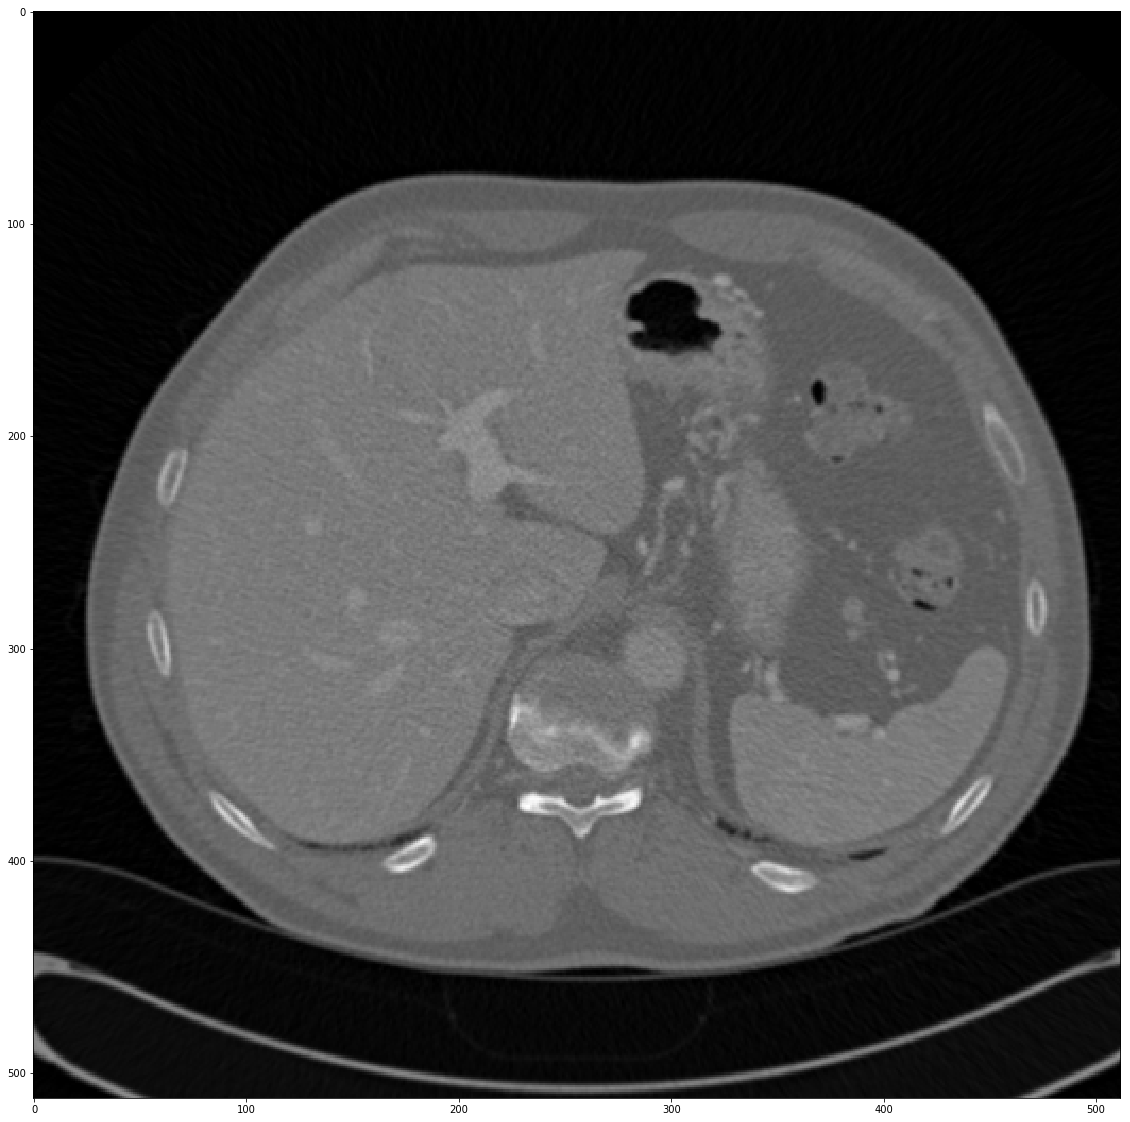
\includegraphics[width=0.3\textwidth]{Images/Liver_org.png}%
    \label{fig:image5}%
    }
    \subfigure[Sau khi chuẩn hóa.]{%
    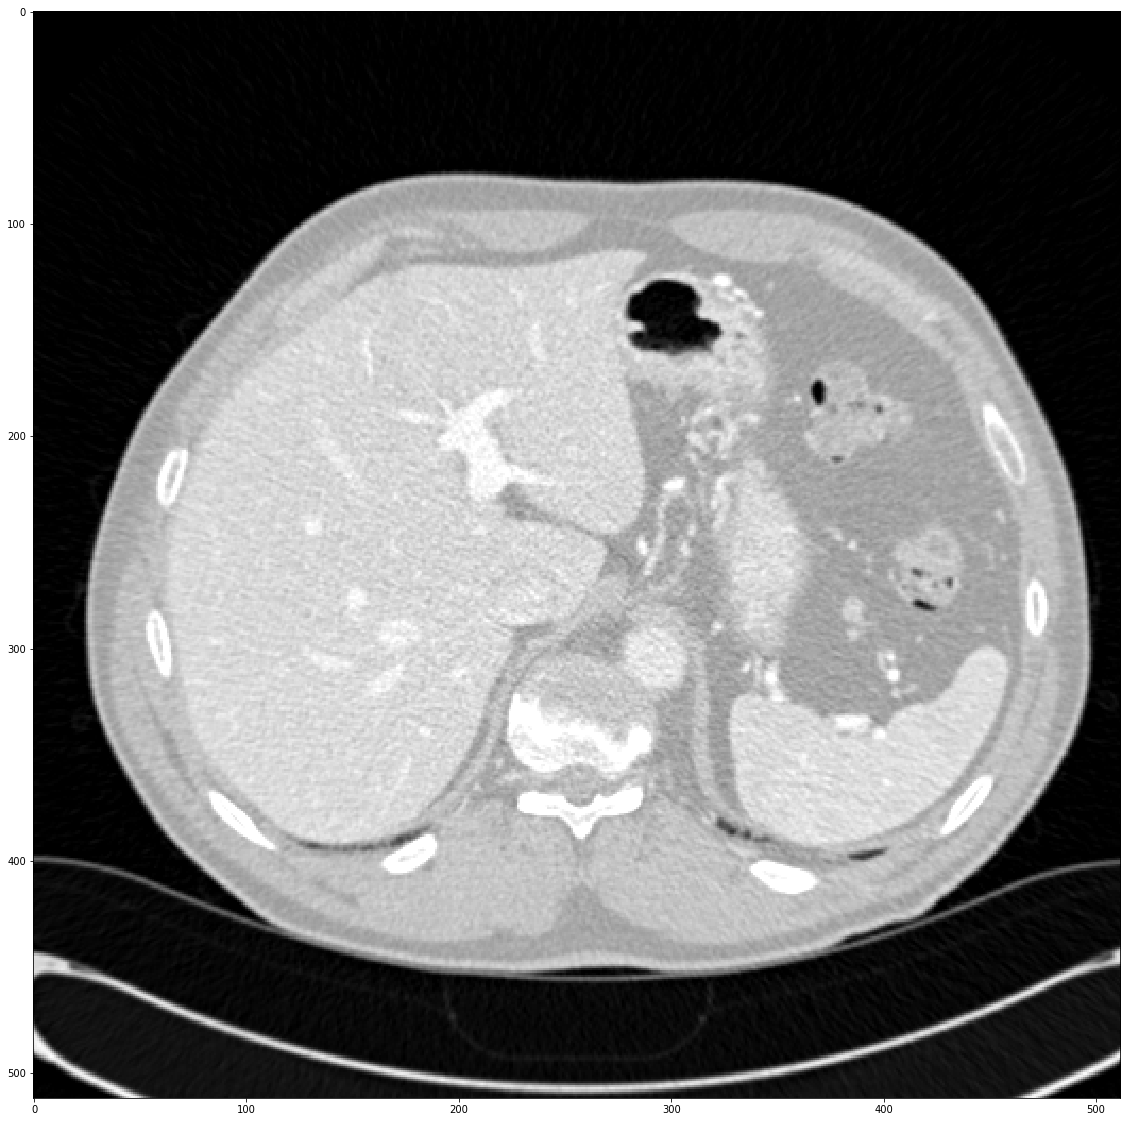
\includegraphics[width=0.3\textwidth]{Images/Liver_norm.png}%
    \label{fig:b}%
    }
    \subfigure[Đã loại bỏ nhiễu.]{%
    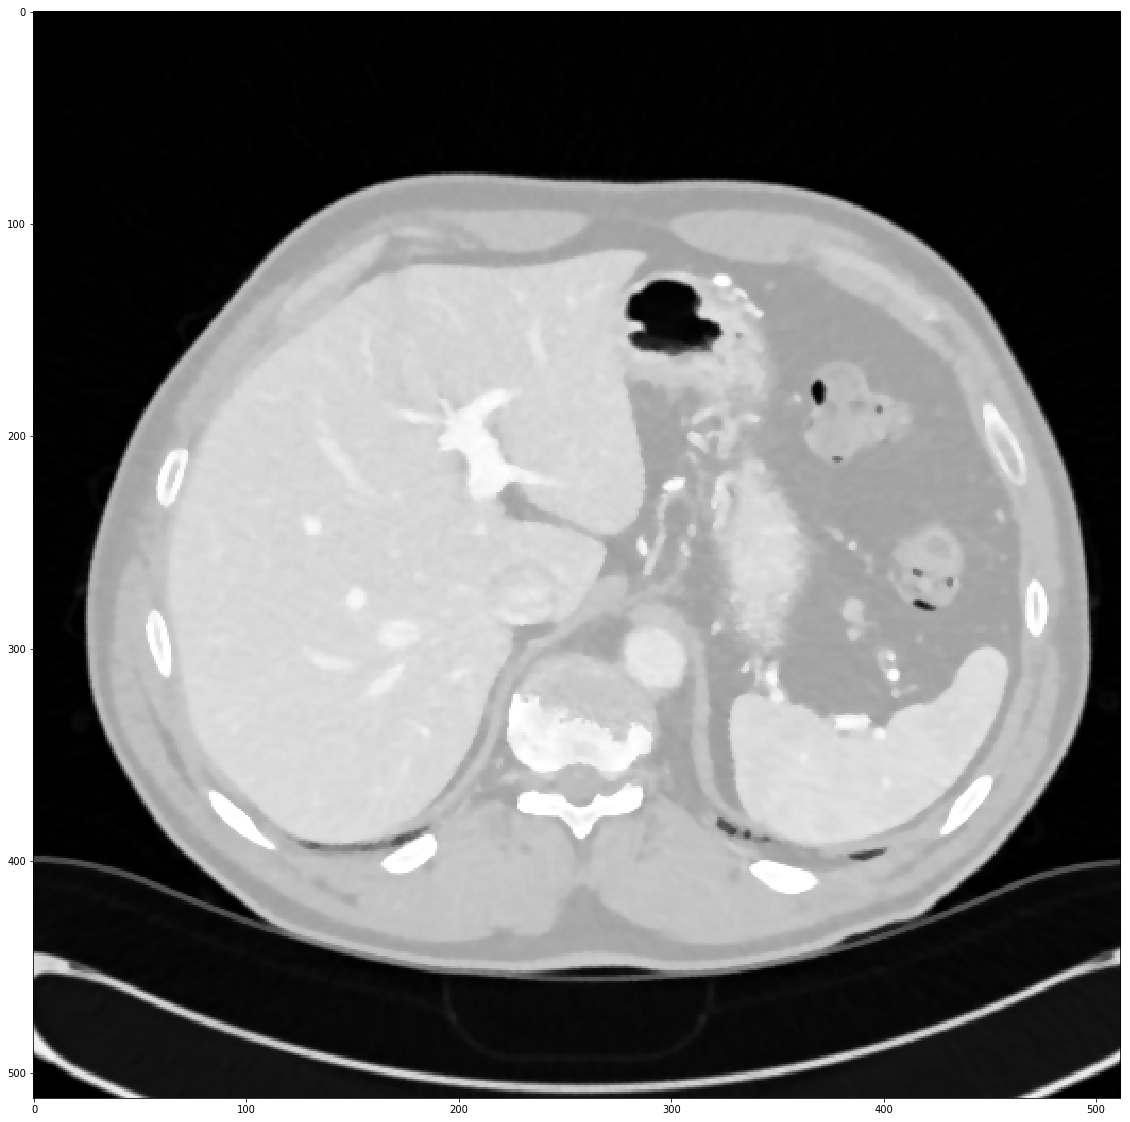
\includegraphics[width=0.3\textwidth]{Images/Liver_rm_noise.png}%
    \label{fig:c}%
    }% 
  \caption{Minh hoạ quá trình tiền xử lý một lát cắt trên ảnh CT}
  \label{fig:ab}
\end{figure*}

\subsection{Loại bỏ nhiễu}
Chúng tôi đã sử dụng công cụ Isotropic diffusion filter trong thư viện SimpleItk để loại bỏ nhiểu. Các tham số sử dụng:
\begin{itemize}
    \item Iterations: 10
    \item TimeStep: 0.625
    \item Conductance Parameter: 1.5
\end{itemize}
\subsection{Isometric}
Dữ liệu trên các tập SLIVER07, 3Dircadb và LITS2017 có khoảng cách giữa các voxel (spacing) rất khác nhau sẽ gây khó khăn cho mô hình phân đoạn. Đặc biệt là khoảng cách giữa các voxels trục Z ứng với khoảng cách giữa các lát cắt nằm trong khoảng rất lớn, từ 0.5 mm đến 6 mm. Vì vậy, chúng tôi đã đồng bộ khoảng cách giữa các voxels trên tất cả các trục về 1 (mm) đối với tất cả các mẫu dữ liệu. Việc này được thực hiện bằng công cụ Zoom trong thư viện Scipy với nội suy Cubic Spline, $Zoom = (Spacing_x, Spacing_y, Spacing_z)$.

